\documentclass[twoside]{book}

% Packages required by doxygen
\usepackage{fixltx2e}
\usepackage{calc}
\usepackage{doxygen}
\usepackage[export]{adjustbox} % also loads graphicx
\usepackage{graphicx}
\usepackage[utf8]{inputenc}
\usepackage{makeidx}
\usepackage{multicol}
\usepackage{multirow}
\PassOptionsToPackage{warn}{textcomp}
\usepackage{textcomp}
\usepackage[nointegrals]{wasysym}
\usepackage[table]{xcolor}

% Font selection
\usepackage[T1]{fontenc}
\usepackage[scaled=.90]{helvet}
\usepackage{courier}
\usepackage{amssymb}
\usepackage{sectsty}
\renewcommand{\familydefault}{\sfdefault}
\allsectionsfont{%
  \fontseries{bc}\selectfont%
  \color{darkgray}%
}
\renewcommand{\DoxyLabelFont}{%
  \fontseries{bc}\selectfont%
  \color{darkgray}%
}
\newcommand{\+}{\discretionary{\mbox{\scriptsize$\hookleftarrow$}}{}{}}

% Page & text layout
\usepackage{geometry}
\geometry{%
  a4paper,%
  top=2.5cm,%
  bottom=2.5cm,%
  left=2.5cm,%
  right=2.5cm%
}
\tolerance=750
\hfuzz=15pt
\hbadness=750
\setlength{\emergencystretch}{15pt}
\setlength{\parindent}{0cm}
\setlength{\parskip}{3ex plus 2ex minus 2ex}
\makeatletter
\renewcommand{\paragraph}{%
  \@startsection{paragraph}{4}{0ex}{-1.0ex}{1.0ex}{%
    \normalfont\normalsize\bfseries\SS@parafont%
  }%
}
\renewcommand{\subparagraph}{%
  \@startsection{subparagraph}{5}{0ex}{-1.0ex}{1.0ex}{%
    \normalfont\normalsize\bfseries\SS@subparafont%
  }%
}
\makeatother

% Headers & footers
\usepackage{fancyhdr}
\pagestyle{fancyplain}
\fancyhead[LE]{\fancyplain{}{\bfseries\thepage}}
\fancyhead[CE]{\fancyplain{}{}}
\fancyhead[RE]{\fancyplain{}{\bfseries\leftmark}}
\fancyhead[LO]{\fancyplain{}{\bfseries\rightmark}}
\fancyhead[CO]{\fancyplain{}{}}
\fancyhead[RO]{\fancyplain{}{\bfseries\thepage}}
\fancyfoot[LE]{\fancyplain{}{}}
\fancyfoot[CE]{\fancyplain{}{}}
\fancyfoot[RE]{\fancyplain{}{\bfseries\scriptsize Generated by Doxygen }}
\fancyfoot[LO]{\fancyplain{}{\bfseries\scriptsize Generated by Doxygen }}
\fancyfoot[CO]{\fancyplain{}{}}
\fancyfoot[RO]{\fancyplain{}{}}
\renewcommand{\footrulewidth}{0.4pt}
\renewcommand{\chaptermark}[1]{%
  \markboth{#1}{}%
}
\renewcommand{\sectionmark}[1]{%
  \markright{\thesection\ #1}%
}

% Indices & bibliography
\usepackage{natbib}
\usepackage[titles]{tocloft}
\setcounter{tocdepth}{3}
\setcounter{secnumdepth}{5}
\makeindex

% Hyperlinks (required, but should be loaded last)
\usepackage{ifpdf}
\ifpdf
  \usepackage[pdftex,pagebackref=true]{hyperref}
\else
  \usepackage[ps2pdf,pagebackref=true]{hyperref}
\fi
\hypersetup{%
  colorlinks=true,%
  linkcolor=blue,%
  citecolor=blue,%
  unicode%
}

% Custom commands
\newcommand{\clearemptydoublepage}{%
  \newpage{\pagestyle{empty}\cleardoublepage}%
}

\usepackage{caption}
\captionsetup{labelsep=space,justification=centering,font={bf},singlelinecheck=off,skip=4pt,position=top}

%===== C O N T E N T S =====

\begin{document}

% Titlepage & ToC
\hypersetup{pageanchor=false,
             bookmarksnumbered=true,
             pdfencoding=unicode
            }
\pagenumbering{roman}
\begin{titlepage}
\vspace*{7cm}
\begin{center}%
{\Large CT kalibracio Arpitol }\\
\vspace*{1cm}
{\large Generated by Doxygen 1.8.11}\\
\end{center}
\end{titlepage}
\clearemptydoublepage
\tableofcontents
\clearemptydoublepage
\pagenumbering{arabic}
\hypersetup{pageanchor=true}

%--- Begin generated contents ---
\chapter{Hierarchical Index}
\section{Class Hierarchy}
This inheritance list is sorted roughly, but not completely, alphabetically\+:\begin{DoxyCompactList}
\item \contentsline{section}{Directory\+Structure\+Converter}{\pageref{classDirectoryStructureConverter}}{}
\item \contentsline{section}{Gaincorr}{\pageref{classGaincorr}}{}
\item \contentsline{section}{gc\+\_\+im\+\_\+container}{\pageref{classgc__im__container}}{}
\item \contentsline{section}{Geomcorr}{\pageref{classGeomcorr}}{}
\item \contentsline{section}{Image\+\_\+cuda\+\_\+compatible}{\pageref{classImage__cuda__compatible}}{}
\begin{DoxyCompactList}
\item \contentsline{section}{Image}{\pageref{classImage}}{}
\end{DoxyCompactList}
\item Q\+Dialog\begin{DoxyCompactList}
\item \contentsline{section}{Coordinate\+Dialog}{\pageref{classCoordinateDialog}}{}
\item \contentsline{section}{geom\+Corr\+Checker\+Dialog}{\pageref{classgeomCorrCheckerDialog}}{}
\end{DoxyCompactList}
\item Q\+Main\+Window\begin{DoxyCompactList}
\item \contentsline{section}{Main\+Window}{\pageref{classMainWindow}}{}
\end{DoxyCompactList}
\item \contentsline{section}{Semaphore\+Set}{\pageref{classSemaphoreSet}}{}
\begin{DoxyCompactList}
\item \contentsline{section}{Semaphore\+Set\+\_\+with\+\_\+\+Timing}{\pageref{classSemaphoreSet__with__Timing}}{}
\end{DoxyCompactList}
\item \contentsline{section}{semun}{\pageref{unionsemun}}{}
\end{DoxyCompactList}

\chapter{Class Index}
\section{Class List}
Here are the classes, structs, unions and interfaces with brief descriptions\+:\begin{DoxyCompactList}
\item\contentsline{section}{\hyperlink{classCoordinateDialog}{Coordinate\+Dialog} }{\pageref{classCoordinateDialog}}{}
\item\contentsline{section}{\hyperlink{classDirectoryStructureConverter}{Directory\+Structure\+Converter} }{\pageref{classDirectoryStructureConverter}}{}
\item\contentsline{section}{\hyperlink{classGaincorr}{Gaincorr} \\*\+: Calculates, contains and reads Gain correction data }{\pageref{classGaincorr}}{}
\item\contentsline{section}{\hyperlink{classgc__im__container}{gc\+\_\+im\+\_\+container} \\*Class to store images before linear fit }{\pageref{classgc__im__container}}{}
\item\contentsline{section}{\hyperlink{classGeomcorr}{Geomcorr} }{\pageref{classGeomcorr}}{}
\item\contentsline{section}{\hyperlink{classgeomCorrCheckerDialog}{geom\+Corr\+Checker\+Dialog} }{\pageref{classgeomCorrCheckerDialog}}{}
\item\contentsline{section}{\hyperlink{classImage}{Image} \\*\+: \hyperlink{classImage}{Image} class that uses QT elements }{\pageref{classImage}}{}
\item\contentsline{section}{\hyperlink{classImage__cuda__compatible}{Image\+\_\+cuda\+\_\+compatible} \\*\+: Stores an image and it\textquotesingle{}s info. Does not use QT related elements }{\pageref{classImage__cuda__compatible}}{}
\item\contentsline{section}{\hyperlink{classMainWindow}{Main\+Window} }{\pageref{classMainWindow}}{}
\item\contentsline{section}{\hyperlink{classSemaphoreSet}{Semaphore\+Set} }{\pageref{classSemaphoreSet}}{}
\item\contentsline{section}{\hyperlink{classSemaphoreSet__with__Timing}{Semaphore\+Set\+\_\+with\+\_\+\+Timing} }{\pageref{classSemaphoreSet__with__Timing}}{}
\item\contentsline{section}{\hyperlink{unionsemun}{semun} }{\pageref{unionsemun}}{}
\end{DoxyCompactList}

\chapter{Class Documentation}
\hypertarget{classCoordinateDialog}{}\section{Coordinate\+Dialog Class Reference}
\label{classCoordinateDialog}\index{Coordinate\+Dialog@{Coordinate\+Dialog}}


Inheritance diagram for Coordinate\+Dialog\+:
\nopagebreak
\begin{figure}[H]
\begin{center}
\leavevmode
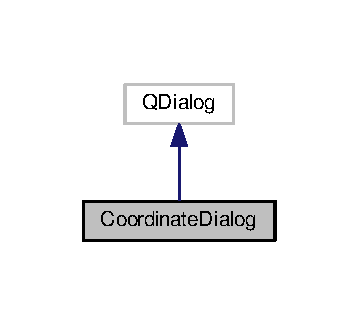
\includegraphics[width=172pt]{classCoordinateDialog__inherit__graph}
\end{center}
\end{figure}


Collaboration diagram for Coordinate\+Dialog\+:
\nopagebreak
\begin{figure}[H]
\begin{center}
\leavevmode
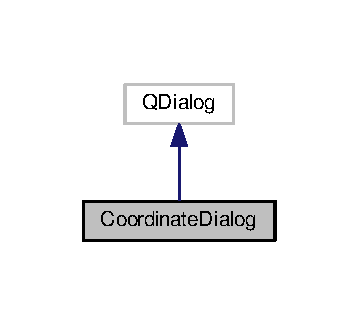
\includegraphics[width=172pt]{classCoordinateDialog__coll__graph}
\end{center}
\end{figure}
\subsection*{Public Member Functions}
\begin{DoxyCompactItemize}
\item 
{\bfseries Coordinate\+Dialog} (Q\+Widget $\ast$parent=0)\hypertarget{classCoordinateDialog_adb54b852402001aaf310b64d7c598846}{}\label{classCoordinateDialog_adb54b852402001aaf310b64d7c598846}

\item 
void {\bfseries setX} (int x)\hypertarget{classCoordinateDialog_a9b05d1ccee4e0c9ddd1d60fc0d3cc080}{}\label{classCoordinateDialog_a9b05d1ccee4e0c9ddd1d60fc0d3cc080}

\item 
void {\bfseries setY} (int y)\hypertarget{classCoordinateDialog_a7dd30911922f73ddd3274364bbfadd9a}{}\label{classCoordinateDialog_a7dd30911922f73ddd3274364bbfadd9a}

\item 
void {\bfseries execute} ()\hypertarget{classCoordinateDialog_a7d5c49c60984e2fa536664e9de317255}{}\label{classCoordinateDialog_a7d5c49c60984e2fa536664e9de317255}

\item 
void {\bfseries getx} (float $\ast$there)\hypertarget{classCoordinateDialog_a49fd02c80700150c4dd608bf78784b95}{}\label{classCoordinateDialog_a49fd02c80700150c4dd608bf78784b95}

\item 
void {\bfseries gety} (float $\ast$there)\hypertarget{classCoordinateDialog_aae06ec512c9b2f7341d1d9974f2468f8}{}\label{classCoordinateDialog_aae06ec512c9b2f7341d1d9974f2468f8}

\item 
void {\bfseries set\+X\+Destination} (float $\ast$x\+Pointer)\hypertarget{classCoordinateDialog_a0ef29e7ef32050b9401db653a1f8525b}{}\label{classCoordinateDialog_a0ef29e7ef32050b9401db653a1f8525b}

\item 
void {\bfseries set\+Y\+Destination} (float $\ast$y\+Pointer)\hypertarget{classCoordinateDialog_a08fbb42162a66cca3f7fe96cfbfc1744}{}\label{classCoordinateDialog_a08fbb42162a66cca3f7fe96cfbfc1744}

\item 
void {\bfseries set\+Label} (Q\+String string)\hypertarget{classCoordinateDialog_af11af9af9ccf1c973f6d7a04226fcf93}{}\label{classCoordinateDialog_af11af9af9ccf1c973f6d7a04226fcf93}

\end{DoxyCompactItemize}


The documentation for this class was generated from the following files\+:\begin{DoxyCompactItemize}
\item 
coordinatedialog.\+h\item 
coordinatedialog.\+cpp\end{DoxyCompactItemize}

\hypertarget{classDirectoryStructureConverter}{}\section{Directory\+Structure\+Converter Class Reference}
\label{classDirectoryStructureConverter}\index{Directory\+Structure\+Converter@{Directory\+Structure\+Converter}}


{\ttfamily \#include $<$directorystructureconverter.\+h$>$}

\subsection*{Public Member Functions}
\begin{DoxyCompactItemize}
\item 
\hyperlink{classDirectoryStructureConverter_accd0d22fdda9e6476dbfe86288d11e92}{Directory\+Structure\+Converter} ()\hypertarget{classDirectoryStructureConverter_accd0d22fdda9e6476dbfe86288d11e92}{}\label{classDirectoryStructureConverter_accd0d22fdda9e6476dbfe86288d11e92}

\begin{DoxyCompactList}\small\item\em This class converts my irectory structure to Toelgyesi\textquotesingle{}s. \end{DoxyCompactList}\item 
void {\bfseries copy\+All} ()\hypertarget{classDirectoryStructureConverter_a61066e6fb5aeed435455add89496586e}{}\label{classDirectoryStructureConverter_a61066e6fb5aeed435455add89496586e}

\item 
void \hyperlink{classDirectoryStructureConverter_aaf899b4074354b0f9fb22be7448f8a36}{copy\+Dir\+As\+Image} ()
\end{DoxyCompactItemize}


\subsection{Detailed Description}
Class to convert directory structure from \char`\"{}every subdir contains images with different settings\char`\"{} to \char`\"{} a single directory contains every image.\char`\"{} 

\subsection{Member Function Documentation}
\index{Directory\+Structure\+Converter@{Directory\+Structure\+Converter}!copy\+Dir\+As\+Image@{copy\+Dir\+As\+Image}}
\index{copy\+Dir\+As\+Image@{copy\+Dir\+As\+Image}!Directory\+Structure\+Converter@{Directory\+Structure\+Converter}}
\subsubsection[{\texorpdfstring{copy\+Dir\+As\+Image()}{copyDirAsImage()}}]{\setlength{\rightskip}{0pt plus 5cm}void Directory\+Structure\+Converter\+::copy\+Dir\+As\+Image (
\begin{DoxyParamCaption}
{}
\end{DoxyParamCaption}
)}\hypertarget{classDirectoryStructureConverter_aaf899b4074354b0f9fb22be7448f8a36}{}\label{classDirectoryStructureConverter_aaf899b4074354b0f9fb22be7448f8a36}
Copies images from subfolders to one folder. Images from a single subfolder are averaged and bads-\/are-\/ignored. 

The documentation for this class was generated from the following files\+:\begin{DoxyCompactItemize}
\item 
directorystructureconverter.\+h\item 
directorystructureconverter.\+cpp\end{DoxyCompactItemize}

\hypertarget{classGaincorr}{}\section{Gaincorr Class Reference}
\label{classGaincorr}\index{Gaincorr@{Gaincorr}}


\+: Calculates, contains and reads Gain correction data  




{\ttfamily \#include $<$gaincorr.\+h$>$}

\subsection*{Public Member Functions}
\begin{DoxyCompactItemize}
\item 
void \hyperlink{classGaincorr_a5751ca7bcc7dca8b298558c65b5fcd50}{read\+And\+Calculate\+Gain} ()
\begin{DoxyCompactList}\small\item\em Reads images to calculate gain correction data. \end{DoxyCompactList}\item 
void \hyperlink{classGaincorr_adae369206efa5a41806749162051b7a9}{read\+And\+Calculate\+Offset} ()
\begin{DoxyCompactList}\small\item\em Reads image files for ofsset calibration, caluclates and saves ofset corrigation data. \end{DoxyCompactList}\item 
void \hyperlink{classGaincorr_abda7eed0445b5590b0dfafd3ca4f58ec}{readgainfactors} ()
\begin{DoxyCompactList}\small\item\em Reads factors for gain correction from files. \end{DoxyCompactList}\item 
void \hyperlink{classGaincorr_af4413aa4ff1c30952e3e3feb30b0beb4}{readoffsetfactors} ()
\begin{DoxyCompactList}\small\item\em Reads offset correction data. \end{DoxyCompactList}\item 
void {\bfseries gaincorrigateimage} (\hyperlink{classImage__cuda__compatible}{Image\+\_\+cuda\+\_\+compatible} \&image)\hypertarget{classGaincorr_a792a26c354754272b251f8c70ca27728}{}\label{classGaincorr_a792a26c354754272b251f8c70ca27728}

\item 
void \hyperlink{classGaincorr_a85f655120337216bb93e18de5807bc11}{offsetcorrigateimage} (\hyperlink{classImage__cuda__compatible}{Image\+\_\+cuda\+\_\+compatible} \&image)
\begin{DoxyCompactList}\small\item\em Offset corrigates the given image. \end{DoxyCompactList}\end{DoxyCompactItemize}


\subsection{Detailed Description}
\+: Calculates, contains and reads Gain correction data 

$<$$<$insert long=\char`\"{}\char`\"{} description=\char`\"{}\char`\"{} here=\char`\"{}\char`\"{}$>$$>$ 

\subsection{Member Function Documentation}
\index{Gaincorr@{Gaincorr}!offsetcorrigateimage@{offsetcorrigateimage}}
\index{offsetcorrigateimage@{offsetcorrigateimage}!Gaincorr@{Gaincorr}}
\subsubsection[{\texorpdfstring{offsetcorrigateimage(\+Image\+\_\+cuda\+\_\+compatible \&image)}{offsetcorrigateimage(Image_cuda_compatible &image)}}]{\setlength{\rightskip}{0pt plus 5cm}void Gaincorr\+::offsetcorrigateimage (
\begin{DoxyParamCaption}
\item[{{\bf Image\+\_\+cuda\+\_\+compatible} \&}]{image}
\end{DoxyParamCaption}
)}\hypertarget{classGaincorr_a85f655120337216bb93e18de5807bc11}{}\label{classGaincorr_a85f655120337216bb93e18de5807bc11}


Offset corrigates the given image. 

\hyperlink{classImage}{Image} is offset corrigated and owerwritten in the memory. \index{Gaincorr@{Gaincorr}!read\+And\+Calculate\+Gain@{read\+And\+Calculate\+Gain}}
\index{read\+And\+Calculate\+Gain@{read\+And\+Calculate\+Gain}!Gaincorr@{Gaincorr}}
\subsubsection[{\texorpdfstring{read\+And\+Calculate\+Gain()}{readAndCalculateGain()}}]{\setlength{\rightskip}{0pt plus 5cm}void Gaincorr\+::read\+And\+Calculate\+Gain (
\begin{DoxyParamCaption}
{}
\end{DoxyParamCaption}
)}\hypertarget{classGaincorr_a5751ca7bcc7dca8b298558c65b5fcd50}{}\label{classGaincorr_a5751ca7bcc7dca8b298558c65b5fcd50}


Reads images to calculate gain correction data. 

The functions asks for an input folder and an output folder. In the input folder, images sould be in subfolders. Every subfolder sould contain one or more image with the same settings (Voltage, Exp time, amperage), with an info file. Images are only loaded from the subfolders of the user given directory. Images are stored in the \hyperlink{classgc__im__container}{gc\+\_\+im\+\_\+container} class, then gain correction data are calculated by linear fitting to offset corrected pixel values in the function of the product of exposition time and amperage. \index{Gaincorr@{Gaincorr}!read\+And\+Calculate\+Offset@{read\+And\+Calculate\+Offset}}
\index{read\+And\+Calculate\+Offset@{read\+And\+Calculate\+Offset}!Gaincorr@{Gaincorr}}
\subsubsection[{\texorpdfstring{read\+And\+Calculate\+Offset()}{readAndCalculateOffset()}}]{\setlength{\rightskip}{0pt plus 5cm}void Gaincorr\+::read\+And\+Calculate\+Offset (
\begin{DoxyParamCaption}
{}
\end{DoxyParamCaption}
)}\hypertarget{classGaincorr_adae369206efa5a41806749162051b7a9}{}\label{classGaincorr_adae369206efa5a41806749162051b7a9}


Reads image files for ofsset calibration, caluclates and saves ofset corrigation data. 

Asks the user for the folder that contains offset correction image set, and another folder to save the offset correction factors. Images should be in the subfolders of the given input folder. Every subolder should contain images with the same exposition time settings. Images are read and then offset corrections factors are determined by linear fit to everry pixel in the function of the exposition time. They are saved in float type binary image files in the output folder, with names offsetslope.\+binf and offsetintercept.\+binf \index{Gaincorr@{Gaincorr}!readgainfactors@{readgainfactors}}
\index{readgainfactors@{readgainfactors}!Gaincorr@{Gaincorr}}
\subsubsection[{\texorpdfstring{readgainfactors()}{readgainfactors()}}]{\setlength{\rightskip}{0pt plus 5cm}void Gaincorr\+::readgainfactors (
\begin{DoxyParamCaption}
{}
\end{DoxyParamCaption}
)}\hypertarget{classGaincorr_abda7eed0445b5590b0dfafd3ca4f58ec}{}\label{classGaincorr_abda7eed0445b5590b0dfafd3ca4f58ec}


Reads factors for gain correction from files. 

Reads slope and intercept files for gain correction. Asks the user to choose a folder. In this folder there should be the files containing slope and intercept data for gain correction. Name format\+: intercept$<$voltage$>$.\+binf and slope$<$voltage$>$.\+binf. Reads every file with the given syntax, and stores them, if both an intercept and a slope file is there for a given voltage. \index{Gaincorr@{Gaincorr}!readoffsetfactors@{readoffsetfactors}}
\index{readoffsetfactors@{readoffsetfactors}!Gaincorr@{Gaincorr}}
\subsubsection[{\texorpdfstring{readoffsetfactors()}{readoffsetfactors()}}]{\setlength{\rightskip}{0pt plus 5cm}void Gaincorr\+::readoffsetfactors (
\begin{DoxyParamCaption}
{}
\end{DoxyParamCaption}
)}\hypertarget{classGaincorr_af4413aa4ff1c30952e3e3feb30b0beb4}{}\label{classGaincorr_af4413aa4ff1c30952e3e3feb30b0beb4}


Reads offset correction data. 

Reads slope and intercept files for offset correction. Asks the user to choose a folder. In this folder there should be the files containing slope and intercept data for offset correction. Name format\+: offsetintercept.\+binf and offsetslope.\+binf. 

The documentation for this class was generated from the following files\+:\begin{DoxyCompactItemize}
\item 
gaincorr.\+h\item 
gaincorr.\+cpp\end{DoxyCompactItemize}

\hypertarget{classgc__im__container}{}\section{gc\+\_\+im\+\_\+container Class Reference}
\label{classgc__im__container}\index{gc\+\_\+im\+\_\+container@{gc\+\_\+im\+\_\+container}}


Class to store images before linear fit.  




{\ttfamily \#include $<$gc\+\_\+im\+\_\+container.\+h$>$}

\subsection*{Public Member Functions}
\begin{DoxyCompactItemize}
\item 
\hyperlink{classgc__im__container_af5a0249e639585c347c80b82615d7e6f}{gc\+\_\+im\+\_\+container} ()\hypertarget{classgc__im__container_af5a0249e639585c347c80b82615d7e6f}{}\label{classgc__im__container_af5a0249e639585c347c80b82615d7e6f}

\begin{DoxyCompactList}\small\item\em Default constructor. \end{DoxyCompactList}\item 
void \hyperlink{classgc__im__container_a90e9cc6f3b17ee36228c9807675bc5ef}{add} (\hyperlink{classImage__cuda__compatible}{Image\+\_\+cuda\+\_\+compatible} \&im)\hypertarget{classgc__im__container_a90e9cc6f3b17ee36228c9807675bc5ef}{}\label{classgc__im__container_a90e9cc6f3b17ee36228c9807675bc5ef}

\begin{DoxyCompactList}\small\item\em Adds in image to the containter. \end{DoxyCompactList}\item 
void \hyperlink{classgc__im__container_a2a58af5fd3ea64a9efe1c632e6e7a111}{clear} ()\hypertarget{classgc__im__container_a2a58af5fd3ea64a9efe1c632e6e7a111}{}\label{classgc__im__container_a2a58af5fd3ea64a9efe1c632e6e7a111}

\begin{DoxyCompactList}\small\item\em Deassings memory. \end{DoxyCompactList}\item 
int \hyperlink{classgc__im__container_af1f0bd117c4691d73178142a156dabec}{getimageno} ()\hypertarget{classgc__im__container_af1f0bd117c4691d73178142a156dabec}{}\label{classgc__im__container_af1f0bd117c4691d73178142a156dabec}

\begin{DoxyCompactList}\small\item\em Returns the number of images in the container. \end{DoxyCompactList}\item 
void \hyperlink{classgc__im__container_a72fe57a7d152a1a8152f9a76062bd9b3}{calculate} (\hyperlink{classImage__cuda__compatible}{Image\+\_\+cuda\+\_\+compatible} \&slope, \hyperlink{classImage__cuda__compatible}{Image\+\_\+cuda\+\_\+compatible} \&intercept)
\end{DoxyCompactItemize}


\subsection{Detailed Description}
Class to store images before linear fit. 

\subsection{Member Function Documentation}
\index{gc\+\_\+im\+\_\+container@{gc\+\_\+im\+\_\+container}!calculate@{calculate}}
\index{calculate@{calculate}!gc\+\_\+im\+\_\+container@{gc\+\_\+im\+\_\+container}}
\subsubsection[{\texorpdfstring{calculate(\+Image\+\_\+cuda\+\_\+compatible \&slope, Image\+\_\+cuda\+\_\+compatible \&intercept)}{calculate(Image_cuda_compatible &slope, Image_cuda_compatible &intercept)}}]{\setlength{\rightskip}{0pt plus 5cm}void gc\+\_\+im\+\_\+container\+::calculate (
\begin{DoxyParamCaption}
\item[{{\bf Image\+\_\+cuda\+\_\+compatible} \&}]{slope, }
\item[{{\bf Image\+\_\+cuda\+\_\+compatible} \&}]{intercept}
\end{DoxyParamCaption}
)}\hypertarget{classgc__im__container_a72fe57a7d152a1a8152f9a76062bd9b3}{}\label{classgc__im__container_a72fe57a7d152a1a8152f9a76062bd9b3}
Fits a line on the image pixel data in the function of exptime$\ast$amperage of the image. Line slope and intercept are stored in the given images. 

The documentation for this class was generated from the following files\+:\begin{DoxyCompactItemize}
\item 
gc\+\_\+im\+\_\+container.\+h\item 
gc\+\_\+im\+\_\+container.\+cpp\end{DoxyCompactItemize}

\hypertarget{classGeomcorr}{}\section{Geomcorr Class Reference}
\label{classGeomcorr}\index{Geomcorr@{Geomcorr}}
\subsection*{Public Member Functions}
\begin{DoxyCompactItemize}
\item 
void {\bfseries extract\+Coordinates} (\hyperlink{classImage__cuda__compatible}{Image\+\_\+cuda\+\_\+compatible} \&image, bool draw\+Only=false, bool onlyN=false)\hypertarget{classGeomcorr_a1c77404e2163d3d3f8d03d932b31ad20}{}\label{classGeomcorr_a1c77404e2163d3d3f8d03d932b31ad20}

\item 
void {\bfseries read\+And\+Calculate\+Geom} ()\hypertarget{classGeomcorr_a083128b51dc70ad6d94536e3f93a459a}{}\label{classGeomcorr_a083128b51dc70ad6d94536e3f93a459a}

\item 
void {\bfseries initialize\+Device\+Vector} (int n, int size, int u)\hypertarget{classGeomcorr_aaa49852e93cfd941148223eee0ddcee5}{}\label{classGeomcorr_aaa49852e93cfd941148223eee0ddcee5}

\item 
void {\bfseries add\+Coordinates} ()\hypertarget{classGeomcorr_a8119f3169e1abe814a5f03bf9fa90486}{}\label{classGeomcorr_a8119f3169e1abe814a5f03bf9fa90486}

\item 
void {\bfseries add\+Coordinates} (\hyperlink{classImage__cuda__compatible}{Image\+\_\+cuda\+\_\+compatible} \&)\hypertarget{classGeomcorr_a95eaae8131a0c9d953b8cf3e331c603c}{}\label{classGeomcorr_a95eaae8131a0c9d953b8cf3e331c603c}

\item 
bool {\bfseries export\+Text} (std\+::string filename)\hypertarget{classGeomcorr_a29d08ee02403ade8e71be177b2b4dd5e}{}\label{classGeomcorr_a29d08ee02403ade8e71be177b2b4dd5e}

\item 
void {\bfseries calculate\+Eta} ()\hypertarget{classGeomcorr_a3ffb751ba6ad0308f4fb60ce80ee106e}{}\label{classGeomcorr_a3ffb751ba6ad0308f4fb60ce80ee106e}

\item 
void {\bfseries fit\+Ellipse} (int i, float $\ast$a, float $\ast$b, float $\ast$c, float $\ast$u, float $\ast$v, double $\ast$error)\hypertarget{classGeomcorr_a2e5a7f6196fa85443c8d61032f610c2f}{}\label{classGeomcorr_a2e5a7f6196fa85443c8d61032f610c2f}

\item 
void {\bfseries fit\+Ellipse\+Wu} (int i, float $\ast$a, float $\ast$b, float $\ast$c, float $\ast$u, float $\ast$v, double $\ast$error)\hypertarget{classGeomcorr_a2af6517ab0310f41125b319c82cffe2f}{}\label{classGeomcorr_a2af6517ab0310f41125b319c82cffe2f}

\item 
int {\bfseries getn} ()\hypertarget{classGeomcorr_a28274f589b43b4953ecb26acabb8f01f}{}\label{classGeomcorr_a28274f589b43b4953ecb26acabb8f01f}

\item 
double {\bfseries calculate\+Phase} (int i, float u)\hypertarget{classGeomcorr_adefc263fdcec001ce78713f041fcb00d}{}\label{classGeomcorr_adefc263fdcec001ce78713f041fcb00d}

\item 
bool {\bfseries coordinates\+To\+C\+PU} (int $\ast$h\+\_\+x, int $\ast$h\+\_\+y, int n)\hypertarget{classGeomcorr_a2db2d333164befead593c6ba9a125d8e}{}\label{classGeomcorr_a2db2d333164befead593c6ba9a125d8e}

\item 
double {\bfseries get\+Eta} ()\hypertarget{classGeomcorr_a98c2856046a11d7f131e09dd1fa0d97b}{}\label{classGeomcorr_a98c2856046a11d7f131e09dd1fa0d97b}

\item 
void {\bfseries d\+And\+V\+With\+Wu} (float $\ast$a, float $\ast$b, float $\ast$v, float $\ast$D, float $\ast$v0)\hypertarget{classGeomcorr_a570f0ec4cd5db6d8d0d97264d2f3afca}{}\label{classGeomcorr_a570f0ec4cd5db6d8d0d97264d2f3afca}

\item 
bool {\bfseries is\+Ball\+On\+Left\+Side} (int i, float u0)\hypertarget{classGeomcorr_a18255dc56f87a2fea7ed927f923bf3d3}{}\label{classGeomcorr_a18255dc56f87a2fea7ed927f923bf3d3}

\end{DoxyCompactItemize}
\subsection*{Friends}
\begin{DoxyCompactItemize}
\item 
class {\bfseries Gaincorr}\hypertarget{classGeomcorr_a851375f64345af5451f69b4299b1b6cc}{}\label{classGeomcorr_a851375f64345af5451f69b4299b1b6cc}

\end{DoxyCompactItemize}


The documentation for this class was generated from the following files\+:\begin{DoxyCompactItemize}
\item 
geomcorr.\+h\item 
geomcorr.\+cpp\end{DoxyCompactItemize}

\hypertarget{classgeomCorrCheckerDialog}{}\section{geom\+Corr\+Checker\+Dialog Class Reference}
\label{classgeomCorrCheckerDialog}\index{geom\+Corr\+Checker\+Dialog@{geom\+Corr\+Checker\+Dialog}}


Inheritance diagram for geom\+Corr\+Checker\+Dialog\+:
\nopagebreak
\begin{figure}[H]
\begin{center}
\leavevmode
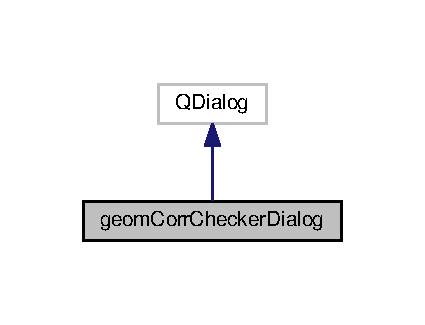
\includegraphics[width=204pt]{classgeomCorrCheckerDialog__inherit__graph}
\end{center}
\end{figure}


Collaboration diagram for geom\+Corr\+Checker\+Dialog\+:
\nopagebreak
\begin{figure}[H]
\begin{center}
\leavevmode
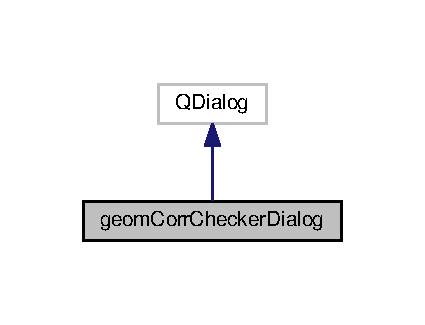
\includegraphics[width=204pt]{classgeomCorrCheckerDialog__coll__graph}
\end{center}
\end{figure}
\subsection*{Public Member Functions}
\begin{DoxyCompactItemize}
\item 
{\bfseries geom\+Corr\+Checker\+Dialog} (Q\+Widget $\ast$parent=0)\hypertarget{classgeomCorrCheckerDialog_ad9bfbbf7c84e264510a724a103fbe103}{}\label{classgeomCorrCheckerDialog_ad9bfbbf7c84e264510a724a103fbe103}

\item 
void {\bfseries get\+File\+List} ()\hypertarget{classgeomCorrCheckerDialog_aea1e154e1cd5180101fb01d1527969e4}{}\label{classgeomCorrCheckerDialog_aea1e154e1cd5180101fb01d1527969e4}

\end{DoxyCompactItemize}


The documentation for this class was generated from the following files\+:\begin{DoxyCompactItemize}
\item 
geomcorrcheckerdialog.\+h\item 
geomcorrcheckerdialog.\+cpp\end{DoxyCompactItemize}

\hypertarget{classImage}{}\section{Image Class Reference}
\label{classImage}\index{Image@{Image}}


\+: \hyperlink{classImage}{Image} class that uses QT elements.  




{\ttfamily \#include $<$image.\+h$>$}



Inheritance diagram for Image\+:
\nopagebreak
\begin{figure}[H]
\begin{center}
\leavevmode
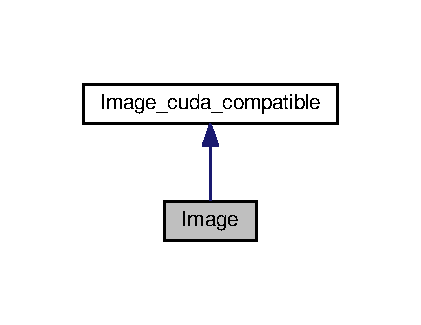
\includegraphics[width=202pt]{classImage__inherit__graph}
\end{center}
\end{figure}


Collaboration diagram for Image\+:
\nopagebreak
\begin{figure}[H]
\begin{center}
\leavevmode
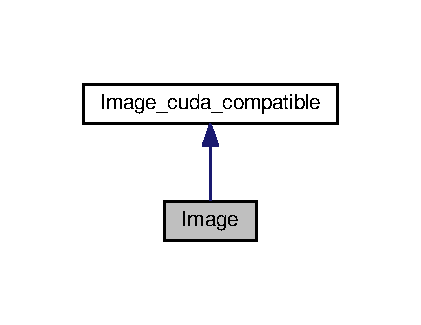
\includegraphics[width=202pt]{classImage__coll__graph}
\end{center}
\end{figure}
\subsection*{Public Member Functions}
\begin{DoxyCompactItemize}
\item 
\hyperlink{classImage_a58edd1c45b4faeb5f789b0d036d02313}{Image} ()\hypertarget{classImage_a58edd1c45b4faeb5f789b0d036d02313}{}\label{classImage_a58edd1c45b4faeb5f789b0d036d02313}

\begin{DoxyCompactList}\small\item\em Default constructor. \end{DoxyCompactList}\item 
\hyperlink{classImage_ada9ac359edb381345fd859b01ada4614}{Image} (\hyperlink{classImage}{Image} const \&image)
\begin{DoxyCompactList}\small\item\em Copy constructor. \end{DoxyCompactList}\item 
void \hyperlink{classImage_a27afd52aa98fe782e4af180dee15d32b}{Qreadfromfile} (Q\+String \hyperlink{classImage__cuda__compatible_a5dbc3fe00b4ca74f9a3868849cb24406}{filename})
\begin{DoxyCompactList}\small\item\em Reads image data from file. Q\+String version. \end{DoxyCompactList}\item 
void \hyperlink{classImage_a306e9ddde48e5bc079cf22676f9ff7d4}{drawimage} (Q\+Label $\ast$label)
\begin{DoxyCompactList}\small\item\em Draws the image to the Q\+Label. \end{DoxyCompactList}\item 
void \hyperlink{classImage_adfb17986907ce55fba5bbc53fa01d686}{writedetailstoscreen} (Q\+Text\+Edit $\ast$text\+Edit)
\begin{DoxyCompactList}\small\item\em Writes technical information to the Q\+Text\+Edit. \end{DoxyCompactList}\end{DoxyCompactItemize}
\subsection*{Additional Inherited Members}


\subsection{Detailed Description}
\+: \hyperlink{classImage}{Image} class that uses QT elements. 

Inherited from image\+\_\+cuda\+\_\+compatible, this class is capable of storing image and it\textquotesingle{}s data as well as it can use QT related functions. It can draw itself and can read itself and it\textquotesingle{}s info from file. 

\subsection{Constructor \& Destructor Documentation}
\index{Image@{Image}!Image@{Image}}
\index{Image@{Image}!Image@{Image}}
\subsubsection[{\texorpdfstring{Image(\+Image const \&image)}{Image(Image const &image)}}]{\setlength{\rightskip}{0pt plus 5cm}Image\+::\+Image (
\begin{DoxyParamCaption}
\item[{{\bf Image} const \&}]{image}
\end{DoxyParamCaption}
)}\hypertarget{classImage_ada9ac359edb381345fd859b01ada4614}{}\label{classImage_ada9ac359edb381345fd859b01ada4614}


Copy constructor. 

copy constructor 

\subsection{Member Function Documentation}
\index{Image@{Image}!drawimage@{drawimage}}
\index{drawimage@{drawimage}!Image@{Image}}
\subsubsection[{\texorpdfstring{drawimage(\+Q\+Label $\ast$label)}{drawimage(QLabel *label)}}]{\setlength{\rightskip}{0pt plus 5cm}void Image\+::drawimage (
\begin{DoxyParamCaption}
\item[{Q\+Label $\ast$}]{label}
\end{DoxyParamCaption}
)}\hypertarget{classImage_a306e9ddde48e5bc079cf22676f9ff7d4}{}\label{classImage_a306e9ddde48e5bc079cf22676f9ff7d4}


Draws the image to the Q\+Label. 

Draws image to Q\+Label. \hyperlink{classImage}{Image} must be read before. \index{Image@{Image}!Qreadfromfile@{Qreadfromfile}}
\index{Qreadfromfile@{Qreadfromfile}!Image@{Image}}
\subsubsection[{\texorpdfstring{Qreadfromfile(\+Q\+String filename)}{Qreadfromfile(QString filename)}}]{\setlength{\rightskip}{0pt plus 5cm}void Image\+::\+Qreadfromfile (
\begin{DoxyParamCaption}
\item[{Q\+String}]{filename}
\end{DoxyParamCaption}
)}\hypertarget{classImage_a27afd52aa98fe782e4af180dee15d32b}{}\label{classImage_a27afd52aa98fe782e4af180dee15d32b}


Reads image data from file. Q\+String version. 

Reads the image from .bin file. \index{Image@{Image}!writedetailstoscreen@{writedetailstoscreen}}
\index{writedetailstoscreen@{writedetailstoscreen}!Image@{Image}}
\subsubsection[{\texorpdfstring{writedetailstoscreen(\+Q\+Text\+Edit $\ast$text\+Edit)}{writedetailstoscreen(QTextEdit *textEdit)}}]{\setlength{\rightskip}{0pt plus 5cm}void Image\+::writedetailstoscreen (
\begin{DoxyParamCaption}
\item[{Q\+Text\+Edit $\ast$}]{text\+Edit}
\end{DoxyParamCaption}
)}\hypertarget{classImage_adfb17986907ce55fba5bbc53fa01d686}{}\label{classImage_adfb17986907ce55fba5bbc53fa01d686}


Writes technical information to the Q\+Text\+Edit. 

Writes the image details to the given Q\+Text\+Edit. Used to debug reasons at the moment. 

The documentation for this class was generated from the following files\+:\begin{DoxyCompactItemize}
\item 
image.\+h\item 
image.\+cpp\end{DoxyCompactItemize}

\hypertarget{classImage__cuda__compatible}{}\section{Image\+\_\+cuda\+\_\+compatible Class Reference}
\label{classImage__cuda__compatible}\index{Image\+\_\+cuda\+\_\+compatible@{Image\+\_\+cuda\+\_\+compatible}}


\+: Stores an image and it\textquotesingle{}s info. Does not use QT related elements.  




{\ttfamily \#include $<$image\+\_\+cuda\+\_\+compatible.\+h$>$}



Inheritance diagram for Image\+\_\+cuda\+\_\+compatible\+:
\nopagebreak
\begin{figure}[H]
\begin{center}
\leavevmode
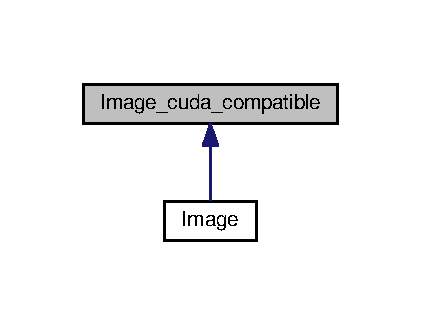
\includegraphics[width=202pt]{classImage__cuda__compatible__inherit__graph}
\end{center}
\end{figure}
\subsection*{Public Member Functions}
\begin{DoxyCompactItemize}
\item 
\hyperlink{classImage__cuda__compatible_acd647640958be8fb9d24f579a5f7aba6}{Image\+\_\+cuda\+\_\+compatible} ()
\begin{DoxyCompactList}\small\item\em Default constructor. \end{DoxyCompactList}\item 
virtual \hyperlink{classImage__cuda__compatible_af56f09a54e75a489f59d8575ace49c9e}{$\sim$\+Image\+\_\+cuda\+\_\+compatible} ()\hypertarget{classImage__cuda__compatible_af56f09a54e75a489f59d8575ace49c9e}{}\label{classImage__cuda__compatible_af56f09a54e75a489f59d8575ace49c9e}

\begin{DoxyCompactList}\small\item\em Destructor. \end{DoxyCompactList}\item 
\hyperlink{classImage__cuda__compatible}{Image\+\_\+cuda\+\_\+compatible} \& \hyperlink{classImage__cuda__compatible_a151b964c26eaefbad2a77fd733321ba8}{operator=} (const \hyperlink{classImage__cuda__compatible}{Image\+\_\+cuda\+\_\+compatible} \&other)\hypertarget{classImage__cuda__compatible_a151b964c26eaefbad2a77fd733321ba8}{}\label{classImage__cuda__compatible_a151b964c26eaefbad2a77fd733321ba8}

\begin{DoxyCompactList}\small\item\em Assigment operator. \end{DoxyCompactList}\item 
\hyperlink{classImage__cuda__compatible}{Image\+\_\+cuda\+\_\+compatible} \& \hyperlink{classImage__cuda__compatible_aaba8e16b5ab9064502f1a18ad36acdbc}{operator+=} (\hyperlink{classImage__cuda__compatible}{Image\+\_\+cuda\+\_\+compatible} \&other)
\begin{DoxyCompactList}\small\item\em Adds another image on the G\+PU. \end{DoxyCompactList}\item 
\hyperlink{classImage__cuda__compatible}{Image\+\_\+cuda\+\_\+compatible} \& \hyperlink{classImage__cuda__compatible_a33ba9942734b6595c75f6e7be54dc975}{operator-\/=} (\hyperlink{classImage__cuda__compatible}{Image\+\_\+cuda\+\_\+compatible} \&other)\hypertarget{classImage__cuda__compatible_a33ba9942734b6595c75f6e7be54dc975}{}\label{classImage__cuda__compatible_a33ba9942734b6595c75f6e7be54dc975}

\begin{DoxyCompactList}\small\item\em Subtracts another image\textquotesingle{}s attributes to this. Also adds pixel values on the G\+PU. \end{DoxyCompactList}\item 
\hyperlink{classImage__cuda__compatible}{Image\+\_\+cuda\+\_\+compatible} \& \hyperlink{classImage__cuda__compatible_adc2d6a2df6470bf1914a1fd2b0a0e49a}{operator$\ast$=} (float n)
\begin{DoxyCompactList}\small\item\em Subtracts another image on the G\+PU. \end{DoxyCompactList}\item 
\hyperlink{classImage__cuda__compatible}{Image\+\_\+cuda\+\_\+compatible} \& \hyperlink{classImage__cuda__compatible_a9ad71725876a14435f64da690950ecd3}{operator/=} (float n)\hypertarget{classImage__cuda__compatible_a9ad71725876a14435f64da690950ecd3}{}\label{classImage__cuda__compatible_a9ad71725876a14435f64da690950ecd3}

\begin{DoxyCompactList}\small\item\em Divides the image with the divisor, on the G\+PU. \end{DoxyCompactList}\item 
void \hyperlink{classImage__cuda__compatible_af5e98d953c3591fe504462e1c1494e19}{equalmax} (\hyperlink{classImage__cuda__compatible}{Image\+\_\+cuda\+\_\+compatible} \&other)\hypertarget{classImage__cuda__compatible_af5e98d953c3591fe504462e1c1494e19}{}\label{classImage__cuda__compatible_af5e98d953c3591fe504462e1c1494e19}

\begin{DoxyCompactList}\small\item\em $<$ Divides an image on the G\+PU. \end{DoxyCompactList}\item 
float {\bfseries correlate\+With} (\hyperlink{classImage__cuda__compatible}{Image\+\_\+cuda\+\_\+compatible} \&other)\hypertarget{classImage__cuda__compatible_a4ddd4869962e4e11eb3937ffb9c5507e}{}\label{classImage__cuda__compatible_a4ddd4869962e4e11eb3937ffb9c5507e}

\item 
void \hyperlink{classImage__cuda__compatible_a99093177f959aeee51732f403be8819e}{clear} ()
\begin{DoxyCompactList}\small\item\em Cleans the image. \end{DoxyCompactList}\item 
void {\bfseries clearwitinradius} (int x, int y, int r)\hypertarget{classImage__cuda__compatible_ab42d33bbe730d570d4db87e911966726}{}\label{classImage__cuda__compatible_ab42d33bbe730d570d4db87e911966726}

\item 
void {\bfseries remove\+\_\+from\+\_\+\+G\+PU} ()\hypertarget{classImage__cuda__compatible_a23d156919fbb8021001049583a4f05bf}{}\label{classImage__cuda__compatible_a23d156919fbb8021001049583a4f05bf}

\item 
void \hyperlink{classImage__cuda__compatible_a249c0b2acafcf79d200a751d186c7159}{calculate\+\_\+meanvalue\+\_\+on\+\_\+\+G\+PU} ()\hypertarget{classImage__cuda__compatible_a249c0b2acafcf79d200a751d186c7159}{}\label{classImage__cuda__compatible_a249c0b2acafcf79d200a751d186c7159}

\begin{DoxyCompactList}\small\item\em Calculates the mean, minimum and maximum value of the image on the G\+PU. \end{DoxyCompactList}\item 
void \hyperlink{classImage__cuda__compatible_a1bc41929e895753fb94d12f3706ed448}{readfromfile} (std\+::string \hyperlink{classImage__cuda__compatible_a5dbc3fe00b4ca74f9a3868849cb24406}{filename})
\begin{DoxyCompactList}\small\item\em Reads image data from file. \end{DoxyCompactList}\item 
void {\bfseries cuda\+Read\+From\+File} (const char $\ast$\hyperlink{classImage__cuda__compatible_a5dbc3fe00b4ca74f9a3868849cb24406}{filename})\hypertarget{classImage__cuda__compatible_a2a22e3122b2f51934449d7024efaf1f2}{}\label{classImage__cuda__compatible_a2a22e3122b2f51934449d7024efaf1f2}

\item 
void \hyperlink{classImage__cuda__compatible_a4cab4c65aced6215d8ce7c5abfd39f47}{cuda\+Read\+From\+Float\+File} (const char $\ast$\hyperlink{classImage__cuda__compatible_a5dbc3fe00b4ca74f9a3868849cb24406}{filename})\hypertarget{classImage__cuda__compatible_a4cab4c65aced6215d8ce7c5abfd39f47}{}\label{classImage__cuda__compatible_a4cab4c65aced6215d8ce7c5abfd39f47}

\begin{DoxyCompactList}\small\item\em Cuda function that copies data from file to G\+PU. \end{DoxyCompactList}\item 
void \hyperlink{classImage__cuda__compatible_ac96a12fbf9cf640638e59d370d0ca6d8}{readfromfloatfile} (std\+::string fname)
\begin{DoxyCompactList}\small\item\em Reads an image from a binary file, containing pixel values as floats. Also reads info file data. \end{DoxyCompactList}\item 
void \hyperlink{classImage__cuda__compatible_a92324b2016515f6eb3996a84017eba4a}{readinfo} ()
\begin{DoxyCompactList}\small\item\em Reads image info from the info file. Info file must be in the same folder as the image. \end{DoxyCompactList}\item 
void {\bfseries writetofile} (std\+::string \hyperlink{classImage__cuda__compatible_a5dbc3fe00b4ca74f9a3868849cb24406}{filename})\hypertarget{classImage__cuda__compatible_af2d4cbc263cfcb4fc09b5a51b7512c9c}{}\label{classImage__cuda__compatible_af2d4cbc263cfcb4fc09b5a51b7512c9c}

\item 
void \hyperlink{classImage__cuda__compatible_a0703a45b3aae00a554fe07d76b85620d}{writetofloatfile} (std\+::string \hyperlink{classImage__cuda__compatible_a5dbc3fe00b4ca74f9a3868849cb24406}{filename})\hypertarget{classImage__cuda__compatible_a0703a45b3aae00a554fe07d76b85620d}{}\label{classImage__cuda__compatible_a0703a45b3aae00a554fe07d76b85620d}

\begin{DoxyCompactList}\small\item\em Writes image values to a binary file, with F\+L\+O\+AT values. \end{DoxyCompactList}\item 
void \hyperlink{classImage__cuda__compatible_a744b4e852b257cf82ae869871bfc90bd}{save\+As\+J\+P\+EG} (std\+::string \hyperlink{classImage__cuda__compatible_a5dbc3fe00b4ca74f9a3868849cb24406}{filename})
\begin{DoxyCompactList}\small\item\em Saves the image as a Jpeg. \end{DoxyCompactList}\item 
void {\bfseries draw\+Cross} (int x, int y, int \hyperlink{classImage__cuda__compatible_a22cea4d1e5568cbea748f48901d99529}{size}=30)\hypertarget{classImage__cuda__compatible_a2f1d26cc2a5fa5d978aff025568fcea2}{}\label{classImage__cuda__compatible_a2f1d26cc2a5fa5d978aff025568fcea2}

\item 
\hyperlink{classImage__cuda__compatible_ac77e1c47ce391c2d9a8caff751c2ac76}{Image\+\_\+cuda\+\_\+compatible} (const \hyperlink{classImage__cuda__compatible}{Image\+\_\+cuda\+\_\+compatible} \&other)
\begin{DoxyCompactList}\small\item\em Copy constructor. \end{DoxyCompactList}\item 
void {\bfseries cuda\+Get\+Short\+Array\+To\+Host} (unsigned short $\ast$h\+\_\+s\+Image)\hypertarget{classImage__cuda__compatible_a01d69f35723a3a6100e0d16538c65d8d}{}\label{classImage__cuda__compatible_a01d69f35723a3a6100e0d16538c65d8d}

\item 
void {\bfseries cuda\+Get\+Array\+To\+Host} (float $\ast$h\+\_\+image)\hypertarget{classImage__cuda__compatible_a693f58d3c9fc76170fe214be6bf21c8f}{}\label{classImage__cuda__compatible_a693f58d3c9fc76170fe214be6bf21c8f}

\item 
void {\bfseries cuda\+Get\+U\+C\+Array\+To\+Host} (unsigned char $\ast$h\+\_\+image)\hypertarget{classImage__cuda__compatible_a7d89ef361f1aefb343c0a8fcea2e5b7d}{}\label{classImage__cuda__compatible_a7d89ef361f1aefb343c0a8fcea2e5b7d}

\item 
void \hyperlink{classImage__cuda__compatible_ac089291fbefec49650fc2b4fe1c8f6d9}{setvoltage} (float f)\hypertarget{classImage__cuda__compatible_ac089291fbefec49650fc2b4fe1c8f6d9}{}\label{classImage__cuda__compatible_ac089291fbefec49650fc2b4fe1c8f6d9}

\begin{DoxyCompactList}\small\item\em Sets the voltage value of the image. \end{DoxyCompactList}\item 
void \hyperlink{classImage__cuda__compatible_a4c4aee34c9aba24c807669a80b3c1805}{setamperage} (float f)\hypertarget{classImage__cuda__compatible_a4c4aee34c9aba24c807669a80b3c1805}{}\label{classImage__cuda__compatible_a4c4aee34c9aba24c807669a80b3c1805}

\begin{DoxyCompactList}\small\item\em Sets the amperage value of the image. \end{DoxyCompactList}\item 
void \hyperlink{classImage__cuda__compatible_a8679a17d852d7d6b009142ae2807c536}{setexptime} (float f)\hypertarget{classImage__cuda__compatible_a8679a17d852d7d6b009142ae2807c536}{}\label{classImage__cuda__compatible_a8679a17d852d7d6b009142ae2807c536}

\begin{DoxyCompactList}\small\item\em Sets the exptime value of the image. \end{DoxyCompactList}\item 
float \hyperlink{classImage__cuda__compatible_a48452a781d574023b87a804e405bf9d9}{getvoltage} ()\hypertarget{classImage__cuda__compatible_a48452a781d574023b87a804e405bf9d9}{}\label{classImage__cuda__compatible_a48452a781d574023b87a804e405bf9d9}

\begin{DoxyCompactList}\small\item\em Returns the voltage of the image. \end{DoxyCompactList}\item 
float \hyperlink{classImage__cuda__compatible_afb0689b067b59712ae4fa4a5713dc80d}{getamperage} ()\hypertarget{classImage__cuda__compatible_afb0689b067b59712ae4fa4a5713dc80d}{}\label{classImage__cuda__compatible_afb0689b067b59712ae4fa4a5713dc80d}

\begin{DoxyCompactList}\small\item\em Returns the amperage of the image. \end{DoxyCompactList}\item 
float \hyperlink{classImage__cuda__compatible_a78ef6fd62bf6b476ba56b188a5f9537b}{getexptime} ()\hypertarget{classImage__cuda__compatible_a78ef6fd62bf6b476ba56b188a5f9537b}{}\label{classImage__cuda__compatible_a78ef6fd62bf6b476ba56b188a5f9537b}

\begin{DoxyCompactList}\small\item\em Returns the exptime of the image. \end{DoxyCompactList}\item 
float \hyperlink{classImage__cuda__compatible_a63a693a97528f4838e1096974a27fafe}{getmean} ()
\item 
float {\bfseries getstdev} ()\hypertarget{classImage__cuda__compatible_ad7cb773d69ee0e8aa102899c68c4f789}{}\label{classImage__cuda__compatible_ad7cb773d69ee0e8aa102899c68c4f789}

\item 
float \hyperlink{classImage__cuda__compatible_a17f7d423caa9ab765fd29befb8929449}{getmax} ()
\item 
float \hyperlink{classImage__cuda__compatible_afcafae2aa9d72108ed15308b52900788}{getmin} ()
\item 
std\+::string \hyperlink{classImage__cuda__compatible_a03f18d23b1196908435e0da143e07c1e}{getid} ()\hypertarget{classImage__cuda__compatible_a03f18d23b1196908435e0da143e07c1e}{}\label{classImage__cuda__compatible_a03f18d23b1196908435e0da143e07c1e}

\begin{DoxyCompactList}\small\item\em Returns the ID of the image. \end{DoxyCompactList}\item 
std\+::string \hyperlink{classImage__cuda__compatible_a6588dcbebccad868403cdd7993cc9f76}{getfilename} ()
\item 
float $\ast$ {\bfseries reserve\+\_\+on\+\_\+\+G\+PU} ()\hypertarget{classImage__cuda__compatible_a9ecba044299f4ced3d44dd9703b52311}{}\label{classImage__cuda__compatible_a9ecba044299f4ced3d44dd9703b52311}

\item 
float $\ast$ {\bfseries copy\+\_\+\+G\+P\+U\+\_\+image} (float $\ast$other)\hypertarget{classImage__cuda__compatible_a4f8384e40c0f012cee04da87d2c43c18}{}\label{classImage__cuda__compatible_a4f8384e40c0f012cee04da87d2c43c18}

\end{DoxyCompactItemize}
\subsection*{Public Attributes}
\begin{DoxyCompactItemize}
\item 
float $\ast$ \hyperlink{classImage__cuda__compatible_aecdcb6343d0b536bae6da90de8d3bc4f}{gpu\+\_\+im}\hypertarget{classImage__cuda__compatible_aecdcb6343d0b536bae6da90de8d3bc4f}{}\label{classImage__cuda__compatible_aecdcb6343d0b536bae6da90de8d3bc4f}

\begin{DoxyCompactList}\small\item\em Poiter to the image on the G\+PU. \end{DoxyCompactList}\end{DoxyCompactItemize}
\subsection*{Static Public Attributes}
\begin{DoxyCompactItemize}
\item 
static const int \hyperlink{classImage__cuda__compatible_add091d9b4be13ea87572c59541d5fe82}{width} = 1536\hypertarget{classImage__cuda__compatible_add091d9b4be13ea87572c59541d5fe82}{}\label{classImage__cuda__compatible_add091d9b4be13ea87572c59541d5fe82}

\begin{DoxyCompactList}\small\item\em Width of the image. Constant among all images. \end{DoxyCompactList}\item 
static const int \hyperlink{classImage__cuda__compatible_abf81de1dbe4a40b6388aabe60ddc5a0c}{height} = 864\hypertarget{classImage__cuda__compatible_abf81de1dbe4a40b6388aabe60ddc5a0c}{}\label{classImage__cuda__compatible_abf81de1dbe4a40b6388aabe60ddc5a0c}

\begin{DoxyCompactList}\small\item\em Height of the image. Constant among all images. \end{DoxyCompactList}\item 
static const long \hyperlink{classImage__cuda__compatible_a22cea4d1e5568cbea748f48901d99529}{size} = 1327104\hypertarget{classImage__cuda__compatible_a22cea4d1e5568cbea748f48901d99529}{}\label{classImage__cuda__compatible_a22cea4d1e5568cbea748f48901d99529}

\begin{DoxyCompactList}\small\item\em Size of the image. Constant among all images. \end{DoxyCompactList}\end{DoxyCompactItemize}
\subsection*{Protected Member Functions}
\begin{DoxyCompactItemize}
\item 
void {\bfseries divide\+\_\+on\+\_\+\+G\+PU} (float divisor)\hypertarget{classImage__cuda__compatible_a4538c764a8101d4008598f2b4fb69c6c}{}\label{classImage__cuda__compatible_a4538c764a8101d4008598f2b4fb69c6c}

\item 
void {\bfseries multiply\+\_\+on\+\_\+\+G\+PU} (float multiplier)\hypertarget{classImage__cuda__compatible_af27e57aacd0ef5381b04cd4298f0996e}{}\label{classImage__cuda__compatible_af27e57aacd0ef5381b04cd4298f0996e}

\item 
void \hyperlink{classImage__cuda__compatible_a5ab957eedf46e3fd9f6deeec0e850e98}{initialize} ()
\begin{DoxyCompactList}\small\item\em Initializes the image. Sets everything to 0 or N\+U\+LL, creates the im array. Used in constructors. \end{DoxyCompactList}\item 
void {\bfseries add\+\_\+on\+\_\+\+G\+PU} (\hyperlink{classImage__cuda__compatible}{Image\+\_\+cuda\+\_\+compatible} \&other)\hypertarget{classImage__cuda__compatible_a3d5049463d7ad72ca1ce89d73a4f446f}{}\label{classImage__cuda__compatible_a3d5049463d7ad72ca1ce89d73a4f446f}

\item 
void {\bfseries subtract\+\_\+on\+\_\+\+G\+PU} (\hyperlink{classImage__cuda__compatible}{Image\+\_\+cuda\+\_\+compatible} \&other)\hypertarget{classImage__cuda__compatible_af766b848ac22ab22717473aaa0f1850c}{}\label{classImage__cuda__compatible_af766b848ac22ab22717473aaa0f1850c}

\end{DoxyCompactItemize}
\subsection*{Protected Attributes}
\begin{DoxyCompactItemize}
\item 
float \hyperlink{classImage__cuda__compatible_ae5bd4f6f3d151170ac091bd102c2a55f}{mean}\hypertarget{classImage__cuda__compatible_ae5bd4f6f3d151170ac091bd102c2a55f}{}\label{classImage__cuda__compatible_ae5bd4f6f3d151170ac091bd102c2a55f}

\begin{DoxyCompactList}\small\item\em Mean value of the image. \end{DoxyCompactList}\item 
float \hyperlink{classImage__cuda__compatible_abb1737b80a69a9ff1937f5f9ac86d3b1}{stdev}\hypertarget{classImage__cuda__compatible_abb1737b80a69a9ff1937f5f9ac86d3b1}{}\label{classImage__cuda__compatible_abb1737b80a69a9ff1937f5f9ac86d3b1}

\begin{DoxyCompactList}\small\item\em Standard deviation. \end{DoxyCompactList}\item 
float {\bfseries max}\hypertarget{classImage__cuda__compatible_a40704256993e1fe59aae1db3c232c213}{}\label{classImage__cuda__compatible_a40704256993e1fe59aae1db3c232c213}

\item 
float {\bfseries min}\hypertarget{classImage__cuda__compatible_a3acbfd922d0073d97edb9f7d03bfbc06}{}\label{classImage__cuda__compatible_a3acbfd922d0073d97edb9f7d03bfbc06}

\item 
float \hyperlink{classImage__cuda__compatible_aa21a71b8308ab320c6d0b8d76220bcd0}{deviation}\hypertarget{classImage__cuda__compatible_aa21a71b8308ab320c6d0b8d76220bcd0}{}\label{classImage__cuda__compatible_aa21a71b8308ab320c6d0b8d76220bcd0}

\begin{DoxyCompactList}\small\item\em Standard deviation of the pixel values. \end{DoxyCompactList}\item 
std\+::string \hyperlink{classImage__cuda__compatible_a5dbc3fe00b4ca74f9a3868849cb24406}{filename}\hypertarget{classImage__cuda__compatible_a5dbc3fe00b4ca74f9a3868849cb24406}{}\label{classImage__cuda__compatible_a5dbc3fe00b4ca74f9a3868849cb24406}

\begin{DoxyCompactList}\small\item\em File name that the image was read from. \end{DoxyCompactList}\item 
std\+::string \hyperlink{classImage__cuda__compatible_a61b0501f13fd930381424ef192264d8c}{directory}\hypertarget{classImage__cuda__compatible_a61b0501f13fd930381424ef192264d8c}{}\label{classImage__cuda__compatible_a61b0501f13fd930381424ef192264d8c}

\begin{DoxyCompactList}\small\item\em Directory name that the image was read from. \end{DoxyCompactList}\item 
std\+::string \hyperlink{classImage__cuda__compatible_ad9b37cc5930be7da0fa1f67944d24c6d}{id}\hypertarget{classImage__cuda__compatible_ad9b37cc5930be7da0fa1f67944d24c6d}{}\label{classImage__cuda__compatible_ad9b37cc5930be7da0fa1f67944d24c6d}

\begin{DoxyCompactList}\small\item\em ID of the image. \end{DoxyCompactList}\item 
float \hyperlink{classImage__cuda__compatible_ad5eb722fdfbacb645668ea2132c5af63}{voltage}\hypertarget{classImage__cuda__compatible_ad5eb722fdfbacb645668ea2132c5af63}{}\label{classImage__cuda__compatible_ad5eb722fdfbacb645668ea2132c5af63}

\begin{DoxyCompactList}\small\item\em Voltage of the X-\/ray tube. \end{DoxyCompactList}\item 
float \hyperlink{classImage__cuda__compatible_a0d99144c0b338d311b5235385c40b63a}{amperage}\hypertarget{classImage__cuda__compatible_a0d99144c0b338d311b5235385c40b63a}{}\label{classImage__cuda__compatible_a0d99144c0b338d311b5235385c40b63a}

\begin{DoxyCompactList}\small\item\em Amperage of the X-\/ray tube. \end{DoxyCompactList}\item 
float \hyperlink{classImage__cuda__compatible_ab6d746eb607f4ce623c069458b2962a2}{exptime}\hypertarget{classImage__cuda__compatible_ab6d746eb607f4ce623c069458b2962a2}{}\label{classImage__cuda__compatible_ab6d746eb607f4ce623c069458b2962a2}

\begin{DoxyCompactList}\small\item\em Exposure time. \end{DoxyCompactList}\end{DoxyCompactItemize}
\subsection*{Friends}
\begin{DoxyCompactItemize}
\item 
class {\bfseries gc\+\_\+im\+\_\+container}\hypertarget{classImage__cuda__compatible_a648c0d5c58a551f0c60469ff653c4030}{}\label{classImage__cuda__compatible_a648c0d5c58a551f0c60469ff653c4030}

\item 
class {\bfseries Gaincorr}\hypertarget{classImage__cuda__compatible_a851375f64345af5451f69b4299b1b6cc}{}\label{classImage__cuda__compatible_a851375f64345af5451f69b4299b1b6cc}

\end{DoxyCompactItemize}


\subsection{Detailed Description}
\+: Stores an image and it\textquotesingle{}s info. Does not use QT related elements. 

Not using QT related elements makes it able to be used in C\+U\+DA. 

\subsection{Constructor \& Destructor Documentation}
\index{Image\+\_\+cuda\+\_\+compatible@{Image\+\_\+cuda\+\_\+compatible}!Image\+\_\+cuda\+\_\+compatible@{Image\+\_\+cuda\+\_\+compatible}}
\index{Image\+\_\+cuda\+\_\+compatible@{Image\+\_\+cuda\+\_\+compatible}!Image\+\_\+cuda\+\_\+compatible@{Image\+\_\+cuda\+\_\+compatible}}
\subsubsection[{\texorpdfstring{Image\+\_\+cuda\+\_\+compatible()}{Image_cuda_compatible()}}]{\setlength{\rightskip}{0pt plus 5cm}Image\+\_\+cuda\+\_\+compatible\+::\+Image\+\_\+cuda\+\_\+compatible (
\begin{DoxyParamCaption}
{}
\end{DoxyParamCaption}
)}\hypertarget{classImage__cuda__compatible_acd647640958be8fb9d24f579a5f7aba6}{}\label{classImage__cuda__compatible_acd647640958be8fb9d24f579a5f7aba6}


Default constructor. 

Constructor. \index{Image\+\_\+cuda\+\_\+compatible@{Image\+\_\+cuda\+\_\+compatible}!Image\+\_\+cuda\+\_\+compatible@{Image\+\_\+cuda\+\_\+compatible}}
\index{Image\+\_\+cuda\+\_\+compatible@{Image\+\_\+cuda\+\_\+compatible}!Image\+\_\+cuda\+\_\+compatible@{Image\+\_\+cuda\+\_\+compatible}}
\subsubsection[{\texorpdfstring{Image\+\_\+cuda\+\_\+compatible(const Image\+\_\+cuda\+\_\+compatible \&other)}{Image_cuda_compatible(const Image_cuda_compatible &other)}}]{\setlength{\rightskip}{0pt plus 5cm}Image\+\_\+cuda\+\_\+compatible\+::\+Image\+\_\+cuda\+\_\+compatible (
\begin{DoxyParamCaption}
\item[{const {\bf Image\+\_\+cuda\+\_\+compatible} \&}]{other}
\end{DoxyParamCaption}
)}\hypertarget{classImage__cuda__compatible_ac77e1c47ce391c2d9a8caff751c2ac76}{}\label{classImage__cuda__compatible_ac77e1c47ce391c2d9a8caff751c2ac76}


Copy constructor. 

Copy Constructor. 

\subsection{Member Function Documentation}
\index{Image\+\_\+cuda\+\_\+compatible@{Image\+\_\+cuda\+\_\+compatible}!clear@{clear}}
\index{clear@{clear}!Image\+\_\+cuda\+\_\+compatible@{Image\+\_\+cuda\+\_\+compatible}}
\subsubsection[{\texorpdfstring{clear()}{clear()}}]{\setlength{\rightskip}{0pt plus 5cm}void Image\+\_\+cuda\+\_\+compatible\+::clear (
\begin{DoxyParamCaption}
{}
\end{DoxyParamCaption}
)}\hypertarget{classImage__cuda__compatible_a99093177f959aeee51732f403be8819e}{}\label{classImage__cuda__compatible_a99093177f959aeee51732f403be8819e}


Cleans the image. 

Sets every variable to default and removes the image from the G\+PU \& the C\+PU. \index{Image\+\_\+cuda\+\_\+compatible@{Image\+\_\+cuda\+\_\+compatible}!getfilename@{getfilename}}
\index{getfilename@{getfilename}!Image\+\_\+cuda\+\_\+compatible@{Image\+\_\+cuda\+\_\+compatible}}
\subsubsection[{\texorpdfstring{getfilename()}{getfilename()}}]{\setlength{\rightskip}{0pt plus 5cm}std\+::string Image\+\_\+cuda\+\_\+compatible\+::getfilename (
\begin{DoxyParamCaption}
{}
\end{DoxyParamCaption}
)}\hypertarget{classImage__cuda__compatible_a6588dcbebccad868403cdd7993cc9f76}{}\label{classImage__cuda__compatible_a6588dcbebccad868403cdd7993cc9f76}
Returns with the filanem of the image. If the image was not read from a file, returns \char`\"{}\char`\"{}. \index{Image\+\_\+cuda\+\_\+compatible@{Image\+\_\+cuda\+\_\+compatible}!getmax@{getmax}}
\index{getmax@{getmax}!Image\+\_\+cuda\+\_\+compatible@{Image\+\_\+cuda\+\_\+compatible}}
\subsubsection[{\texorpdfstring{getmax()}{getmax()}}]{\setlength{\rightskip}{0pt plus 5cm}float Image\+\_\+cuda\+\_\+compatible\+::getmax (
\begin{DoxyParamCaption}
{}
\end{DoxyParamCaption}
)}\hypertarget{classImage__cuda__compatible_a17f7d423caa9ab765fd29befb8929449}{}\label{classImage__cuda__compatible_a17f7d423caa9ab765fd29befb8929449}
Returns the maximum intensity of the image. If the maximum intensity value is not yet calculated,, calculates it. \index{Image\+\_\+cuda\+\_\+compatible@{Image\+\_\+cuda\+\_\+compatible}!getmean@{getmean}}
\index{getmean@{getmean}!Image\+\_\+cuda\+\_\+compatible@{Image\+\_\+cuda\+\_\+compatible}}
\subsubsection[{\texorpdfstring{getmean()}{getmean()}}]{\setlength{\rightskip}{0pt plus 5cm}float Image\+\_\+cuda\+\_\+compatible\+::getmean (
\begin{DoxyParamCaption}
{}
\end{DoxyParamCaption}
)}\hypertarget{classImage__cuda__compatible_a63a693a97528f4838e1096974a27fafe}{}\label{classImage__cuda__compatible_a63a693a97528f4838e1096974a27fafe}
Returns the mean of the image. If the mean value is not yet calculated ( or it is 0), (re)calculates it. \index{Image\+\_\+cuda\+\_\+compatible@{Image\+\_\+cuda\+\_\+compatible}!getmin@{getmin}}
\index{getmin@{getmin}!Image\+\_\+cuda\+\_\+compatible@{Image\+\_\+cuda\+\_\+compatible}}
\subsubsection[{\texorpdfstring{getmin()}{getmin()}}]{\setlength{\rightskip}{0pt plus 5cm}float Image\+\_\+cuda\+\_\+compatible\+::getmin (
\begin{DoxyParamCaption}
{}
\end{DoxyParamCaption}
)}\hypertarget{classImage__cuda__compatible_afcafae2aa9d72108ed15308b52900788}{}\label{classImage__cuda__compatible_afcafae2aa9d72108ed15308b52900788}
Returns the minimum intensity of the image. If the minimum intensity value is not yet calculated ( or it is 0), (re)calculates it. \index{Image\+\_\+cuda\+\_\+compatible@{Image\+\_\+cuda\+\_\+compatible}!initialize@{initialize}}
\index{initialize@{initialize}!Image\+\_\+cuda\+\_\+compatible@{Image\+\_\+cuda\+\_\+compatible}}
\subsubsection[{\texorpdfstring{initialize()}{initialize()}}]{\setlength{\rightskip}{0pt plus 5cm}void Image\+\_\+cuda\+\_\+compatible\+::initialize (
\begin{DoxyParamCaption}
{}
\end{DoxyParamCaption}
)\hspace{0.3cm}{\ttfamily [protected]}}\hypertarget{classImage__cuda__compatible_a5ab957eedf46e3fd9f6deeec0e850e98}{}\label{classImage__cuda__compatible_a5ab957eedf46e3fd9f6deeec0e850e98}


Initializes the image. Sets everything to 0 or N\+U\+LL, creates the im array. Used in constructors. 

Initializes the image. Set\textquotesingle{}s everything to 0. Memory is not assigned. Use only in ctor! \index{Image\+\_\+cuda\+\_\+compatible@{Image\+\_\+cuda\+\_\+compatible}!operator$\ast$=@{operator$\ast$=}}
\index{operator$\ast$=@{operator$\ast$=}!Image\+\_\+cuda\+\_\+compatible@{Image\+\_\+cuda\+\_\+compatible}}
\subsubsection[{\texorpdfstring{operator$\ast$=(float n)}{operator*=(float n)}}]{\setlength{\rightskip}{0pt plus 5cm}{\bf Image\+\_\+cuda\+\_\+compatible} \& Image\+\_\+cuda\+\_\+compatible\+::operator$\ast$= (
\begin{DoxyParamCaption}
\item[{float}]{n}
\end{DoxyParamCaption}
)}\hypertarget{classImage__cuda__compatible_adc2d6a2df6470bf1914a1fd2b0a0e49a}{}\label{classImage__cuda__compatible_adc2d6a2df6470bf1914a1fd2b0a0e49a}


Subtracts another image on the G\+PU. 

Multiplies with a float, on the G\+PU. \index{Image\+\_\+cuda\+\_\+compatible@{Image\+\_\+cuda\+\_\+compatible}!operator+=@{operator+=}}
\index{operator+=@{operator+=}!Image\+\_\+cuda\+\_\+compatible@{Image\+\_\+cuda\+\_\+compatible}}
\subsubsection[{\texorpdfstring{operator+=(\+Image\+\_\+cuda\+\_\+compatible \&other)}{operator+=(Image_cuda_compatible &other)}}]{\setlength{\rightskip}{0pt plus 5cm}{\bf Image\+\_\+cuda\+\_\+compatible} \& Image\+\_\+cuda\+\_\+compatible\+::operator+= (
\begin{DoxyParamCaption}
\item[{{\bf Image\+\_\+cuda\+\_\+compatible} \&}]{other}
\end{DoxyParamCaption}
)}\hypertarget{classImage__cuda__compatible_aaba8e16b5ab9064502f1a18ad36acdbc}{}\label{classImage__cuda__compatible_aaba8e16b5ab9064502f1a18ad36acdbc}


Adds another image on the G\+PU. 

Operator for addition. Adds another image\textquotesingle{}s attributes to this. Also adds pixel values on the G\+PU. \index{Image\+\_\+cuda\+\_\+compatible@{Image\+\_\+cuda\+\_\+compatible}!readfromfile@{readfromfile}}
\index{readfromfile@{readfromfile}!Image\+\_\+cuda\+\_\+compatible@{Image\+\_\+cuda\+\_\+compatible}}
\subsubsection[{\texorpdfstring{readfromfile(std\+::string filename)}{readfromfile(std::string filename)}}]{\setlength{\rightskip}{0pt plus 5cm}void Image\+\_\+cuda\+\_\+compatible\+::readfromfile (
\begin{DoxyParamCaption}
\item[{std\+::string}]{filename}
\end{DoxyParamCaption}
)}\hypertarget{classImage__cuda__compatible_a1bc41929e895753fb94d12f3706ed448}{}\label{classImage__cuda__compatible_a1bc41929e895753fb94d12f3706ed448}


Reads image data from file. 

Reads an image from a binary file, containing pixel values as unsigned integers. Also reads info file data. \index{Image\+\_\+cuda\+\_\+compatible@{Image\+\_\+cuda\+\_\+compatible}!readfromfloatfile@{readfromfloatfile}}
\index{readfromfloatfile@{readfromfloatfile}!Image\+\_\+cuda\+\_\+compatible@{Image\+\_\+cuda\+\_\+compatible}}
\subsubsection[{\texorpdfstring{readfromfloatfile(std\+::string fname)}{readfromfloatfile(std::string fname)}}]{\setlength{\rightskip}{0pt plus 5cm}void Image\+\_\+cuda\+\_\+compatible\+::readfromfloatfile (
\begin{DoxyParamCaption}
\item[{std\+::string}]{fname}
\end{DoxyParamCaption}
)}\hypertarget{classImage__cuda__compatible_ac96a12fbf9cf640638e59d370d0ca6d8}{}\label{classImage__cuda__compatible_ac96a12fbf9cf640638e59d370d0ca6d8}


Reads an image from a binary file, containing pixel values as floats. Also reads info file data. 

\hyperlink{classImage}{Image} is put to the C\+PU memory. \index{Image\+\_\+cuda\+\_\+compatible@{Image\+\_\+cuda\+\_\+compatible}!readinfo@{readinfo}}
\index{readinfo@{readinfo}!Image\+\_\+cuda\+\_\+compatible@{Image\+\_\+cuda\+\_\+compatible}}
\subsubsection[{\texorpdfstring{readinfo()}{readinfo()}}]{\setlength{\rightskip}{0pt plus 5cm}void Image\+\_\+cuda\+\_\+compatible\+::readinfo (
\begin{DoxyParamCaption}
{}
\end{DoxyParamCaption}
)}\hypertarget{classImage__cuda__compatible_a92324b2016515f6eb3996a84017eba4a}{}\label{classImage__cuda__compatible_a92324b2016515f6eb3996a84017eba4a}


Reads image info from the info file. Info file must be in the same folder as the image. 

Reads data from the info file for the specified image. \index{Image\+\_\+cuda\+\_\+compatible@{Image\+\_\+cuda\+\_\+compatible}!save\+As\+J\+P\+EG@{save\+As\+J\+P\+EG}}
\index{save\+As\+J\+P\+EG@{save\+As\+J\+P\+EG}!Image\+\_\+cuda\+\_\+compatible@{Image\+\_\+cuda\+\_\+compatible}}
\subsubsection[{\texorpdfstring{save\+As\+J\+P\+E\+G(std\+::string filename)}{saveAsJPEG(std::string filename)}}]{\setlength{\rightskip}{0pt plus 5cm}void Image\+\_\+cuda\+\_\+compatible\+::save\+As\+J\+P\+EG (
\begin{DoxyParamCaption}
\item[{std\+::string}]{filename}
\end{DoxyParamCaption}
)}\hypertarget{classImage__cuda__compatible_a744b4e852b257cf82ae869871bfc90bd}{}\label{classImage__cuda__compatible_a744b4e852b257cf82ae869871bfc90bd}


Saves the image as a Jpeg. 

It can actually save any Qt supported format, filename extension determines the image type. 

The documentation for this class was generated from the following files\+:\begin{DoxyCompactItemize}
\item 
image\+\_\+cuda\+\_\+compatible.\+h\item 
image\+\_\+cuda\+\_\+compatible.\+cpp\end{DoxyCompactItemize}

\hypertarget{classMainWindow}{}\section{Main\+Window Class Reference}
\label{classMainWindow}\index{Main\+Window@{Main\+Window}}


Inheritance diagram for Main\+Window\+:
\nopagebreak
\begin{figure}[H]
\begin{center}
\leavevmode
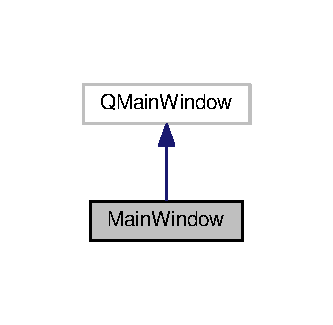
\includegraphics[width=160pt]{classMainWindow__inherit__graph}
\end{center}
\end{figure}


Collaboration diagram for Main\+Window\+:
\nopagebreak
\begin{figure}[H]
\begin{center}
\leavevmode
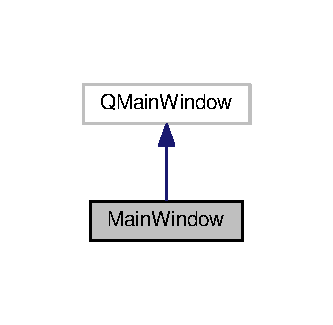
\includegraphics[width=160pt]{classMainWindow__coll__graph}
\end{center}
\end{figure}
\subsection*{Public Member Functions}
\begin{DoxyCompactItemize}
\item 
{\bfseries Main\+Window} (Q\+Widget $\ast$parent=0)\hypertarget{classMainWindow_a8b244be8b7b7db1b08de2a2acb9409db}{}\label{classMainWindow_a8b244be8b7b7db1b08de2a2acb9409db}

\end{DoxyCompactItemize}


The documentation for this class was generated from the following files\+:\begin{DoxyCompactItemize}
\item 
mainwindow.\+h\item 
mainwindow.\+cpp\end{DoxyCompactItemize}

\hypertarget{classSemaphoreSet}{}\section{Semaphore\+Set Class Reference}
\label{classSemaphoreSet}\index{Semaphore\+Set@{Semaphore\+Set}}


Inheritance diagram for Semaphore\+Set\+:
\nopagebreak
\begin{figure}[H]
\begin{center}
\leavevmode
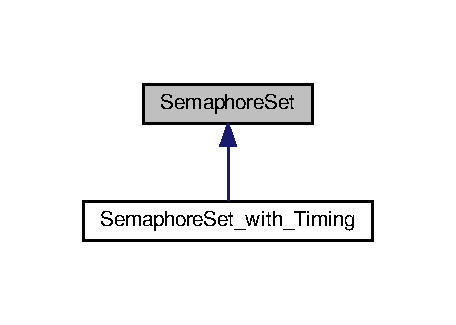
\includegraphics[width=219pt]{classSemaphoreSet__inherit__graph}
\end{center}
\end{figure}
\subsection*{Public Member Functions}
\begin{DoxyCompactItemize}
\item 
{\bfseries Semaphore\+Set} (std\+::string path, int semaphore\+Num)\hypertarget{classSemaphoreSet_a6027ad2c747297e727be26e4eabe2fa8}{}\label{classSemaphoreSet_a6027ad2c747297e727be26e4eabe2fa8}

\item 
virtual int {\bfseries lock} ()\hypertarget{classSemaphoreSet_a466e8fbc146c9fce6a2e81aceaff79c7}{}\label{classSemaphoreSet_a466e8fbc146c9fce6a2e81aceaff79c7}

\item 
virtual int {\bfseries lock\+Specific} (const int index)\hypertarget{classSemaphoreSet_a3624d9c3402e790f3bcd8f2a5f28fa52}{}\label{classSemaphoreSet_a3624d9c3402e790f3bcd8f2a5f28fa52}

\item 
virtual void {\bfseries unlock} ()\hypertarget{classSemaphoreSet_a8205a491451929feac9494341fa870a3}{}\label{classSemaphoreSet_a8205a491451929feac9494341fa870a3}

\item 
void {\bfseries print} ()\hypertarget{classSemaphoreSet_af02b517be7efef6c5baebcf75391d757}{}\label{classSemaphoreSet_af02b517be7efef6c5baebcf75391d757}

\end{DoxyCompactItemize}
\subsection*{Protected Member Functions}
\begin{DoxyCompactItemize}
\item 
bool {\bfseries lock} (int semaphore)\hypertarget{classSemaphoreSet_afeab9e90c4ee63c161159b1d65c9b2be}{}\label{classSemaphoreSet_afeab9e90c4ee63c161159b1d65c9b2be}

\end{DoxyCompactItemize}


The documentation for this class was generated from the following files\+:\begin{DoxyCompactItemize}
\item 
Semaphore\+Set.\+h\item 
Semaphore\+Set.\+cpp\end{DoxyCompactItemize}

\hypertarget{classSemaphoreSet__with__Timing}{}\section{Semaphore\+Set\+\_\+with\+\_\+\+Timing Class Reference}
\label{classSemaphoreSet__with__Timing}\index{Semaphore\+Set\+\_\+with\+\_\+\+Timing@{Semaphore\+Set\+\_\+with\+\_\+\+Timing}}


Inheritance diagram for Semaphore\+Set\+\_\+with\+\_\+\+Timing\+:
\nopagebreak
\begin{figure}[H]
\begin{center}
\leavevmode
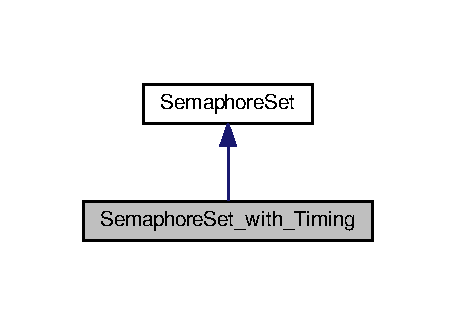
\includegraphics[width=219pt]{classSemaphoreSet__with__Timing__inherit__graph}
\end{center}
\end{figure}


Collaboration diagram for Semaphore\+Set\+\_\+with\+\_\+\+Timing\+:
\nopagebreak
\begin{figure}[H]
\begin{center}
\leavevmode
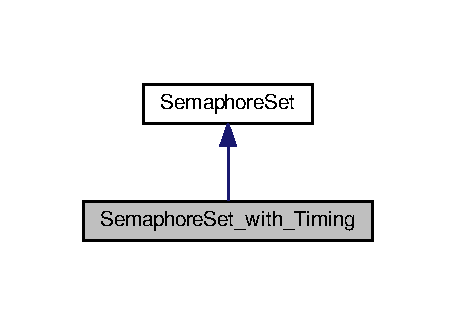
\includegraphics[width=219pt]{classSemaphoreSet__with__Timing__coll__graph}
\end{center}
\end{figure}
\subsection*{Public Member Functions}
\begin{DoxyCompactItemize}
\item 
{\bfseries Semaphore\+Set\+\_\+with\+\_\+\+Timing} (std\+::string path, int semaphore\+Num)\hypertarget{classSemaphoreSet__with__Timing_ab9ab6cf0bdb9385be18444db84611378}{}\label{classSemaphoreSet__with__Timing_ab9ab6cf0bdb9385be18444db84611378}

\item 
virtual int {\bfseries lock} ()\hypertarget{classSemaphoreSet__with__Timing_ad0094fa75fbc904182db64452bc6d5bb}{}\label{classSemaphoreSet__with__Timing_ad0094fa75fbc904182db64452bc6d5bb}

\item 
virtual int {\bfseries lock\+Specific} (const int index)\hypertarget{classSemaphoreSet__with__Timing_a6905ecc96bb6a7cc3ecb439624adfa04}{}\label{classSemaphoreSet__with__Timing_a6905ecc96bb6a7cc3ecb439624adfa04}

\item 
virtual void {\bfseries unlock} ()\hypertarget{classSemaphoreSet__with__Timing_ae47a0e2807c8adfb1a8c1dd03ecb7771}{}\label{classSemaphoreSet__with__Timing_ae47a0e2807c8adfb1a8c1dd03ecb7771}

\item 
double {\bfseries locked\+Time} ()\hypertarget{classSemaphoreSet__with__Timing_a4254bbd58032a3f60d7590c834ba1843}{}\label{classSemaphoreSet__with__Timing_a4254bbd58032a3f60d7590c834ba1843}

\end{DoxyCompactItemize}
\subsection*{Additional Inherited Members}


The documentation for this class was generated from the following files\+:\begin{DoxyCompactItemize}
\item 
Semaphore\+Set.\+h\item 
Semaphore\+Set.\+cpp\end{DoxyCompactItemize}

\hypertarget{unionsemun}{}\section{semun Union Reference}
\label{unionsemun}\index{semun@{semun}}
\subsection*{Public Attributes}
\begin{DoxyCompactItemize}
\item 
int {\bfseries val}\hypertarget{unionsemun_ac6121ecb6d04a024e07e12bd71b94031}{}\label{unionsemun_ac6121ecb6d04a024e07e12bd71b94031}

\item 
struct semid\+\_\+ds $\ast$ {\bfseries buf}\hypertarget{unionsemun_ac6b6428d07d4147fd2cc698b53555bed}{}\label{unionsemun_ac6b6428d07d4147fd2cc698b53555bed}

\item 
unsigned short int $\ast$ {\bfseries array}\hypertarget{unionsemun_ab6029cc01ffece038873310b5adede70}{}\label{unionsemun_ab6029cc01ffece038873310b5adede70}

\item 
struct seminfo $\ast$ {\bfseries \+\_\+\+\_\+buf}\hypertarget{unionsemun_aa0ac6a1a9174a4ae355bc367e7e64780}{}\label{unionsemun_aa0ac6a1a9174a4ae355bc367e7e64780}

\end{DoxyCompactItemize}


The documentation for this union was generated from the following file\+:\begin{DoxyCompactItemize}
\item 
Semaphore\+Set.\+cpp\end{DoxyCompactItemize}

%--- End generated contents ---

% Index
\backmatter
\newpage
\phantomsection
\clearemptydoublepage
\addcontentsline{toc}{chapter}{Index}
\printindex

\end{document}
